
\chapter{Hierarchical mesh refinement with local time step}
\label{mesh_refinement}


Keeping the time step under a certain value relative to the element size in transitory problems is of key importance to achieve good results. Otherwise, an excessively large time step could resort on an over-diffusive solution.
Furthermore, the element size is governed by the physics, it has to be small enough to capture the modes of interest. It is a usual practice to refine the mesh near the region of interest or where the solution is changing rapidly. consequently, the local reduction of the mesh size is imposing a global reduction of the time step.

This section seeks for a strategy with \emph{Local Time Step} (LTS). The main idea consists on adding subdomains characterized by smaller mesh sizes. Thus, a hierarchic mesh refinement is defined with a characteristic mesh size and its corresponding time step. The hierarchical refinement allows to use both non-conforming discretization at space and time level. The only requirement is having a natural number of divisions in order to perform a communication at the coarse level. Figure \ref{multilevel_refinement} shows a hierarchical spatial refinement.

This framework eases the refinement and coarsening procedures. The coarsening process is specially simple, since it consists just on removing elements from the lowest level without having to rebuild the connectivities. On the other hand, a procedure must be defined for the hanging nodes at the boundary and the hanging time steps.



\begin{figure}
    \centering
    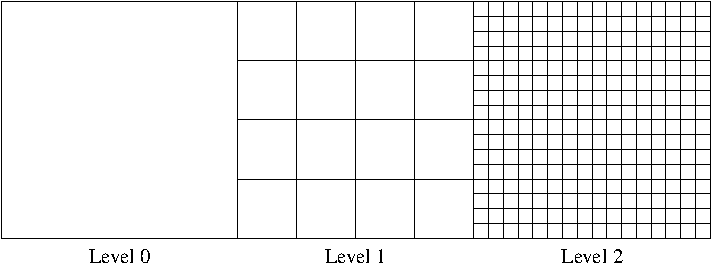
\includegraphics[width=.8\textwidth]{img/multigrid/multilevel_refinement.pdf}
    \caption{Two refinement levels. Each refinement has two levels of sub divisions.}
    \label{multilevel_refinement}
\end{figure}



There have been previous advances in LTS. An early proposal can be found in \cite{chevalier1997}, where a LTS was proposed for waves propagation using the Maxwell's equations. The main interest of the LTS is the reduction of computational resources and to avoid the numerical diffusion caused by small time steps on coarse regions of the mesh. The cost of introducing a LTS with local mesh refinement is an instability at the coarse-fine interface. Collino analyzed the LTS for the hyperbolic 1D equations in \cite{collino2003a,collino2003b} and overcame this instability analyzing the conservation of the discrete energy through refinement levels. Usually the LTS has been linked to explicit time steps.

DG have been successfully applied to overcome the stability constraint of explicit LTS. For example, in \cite{diaz2009} the non-conforming properties of DG are exploited to ensure stability. In that case, the continuity is enforced by the so-called numerical fluxes arising from the non conforming discretization of DG. On the other hand, CG is still a good solution, in \cite{almquist2016} stability is ensured by the classical technique of overlapping one coarse element with the fine mesh. A similar example can be found in \cite{grote2021}.

Finally, the most recent studies move towards massively parallel implementation. In \cite{baiges2016} a new library is presented. In this appendix, the implementation is designed in parallel processing, but without memory parallelization. On the other hand, attention is devoted to the algorithm, which is fully decoupled from the time integration, allowing for implicit or explicit schemes. In the future, this procedure could be easily extended to shared memory parallelization.


\section{Algorithm}

As stated in \cite{almquist2016,collino2003a}, the time step is driven by the finest mesh and the stability condition arising from the coarse-fine interface is overcome with a partial overlap. In the present case, the choice is to have a hierarchical structure of refined meshes fully overlapped, see Figure \ref{multilevel_overlap}. Apart from the advantages in parallel implementation, it allows to fully decouple the LTS from the time integration.

Having several meshes overlapped has an extra cost, since the coarse mesh has to be computed with the coarse time step at the refined region. However, its computational cost is insignificant in comparison with the resolution of the fine level. This step is considered as a predictor and is necessary for applying the boundary conditions at the fine level.

Hence, the stability relies on the boundary conditions applied to the fine level. The boundary conditions stated in chapter \ref{equations} does not necessary link all the variables, thus, some of the unknowns might not be continuous across the coarse-fine interface. This is the cost to pay for stability.

\begin{figure} [htpb]
    \centering
    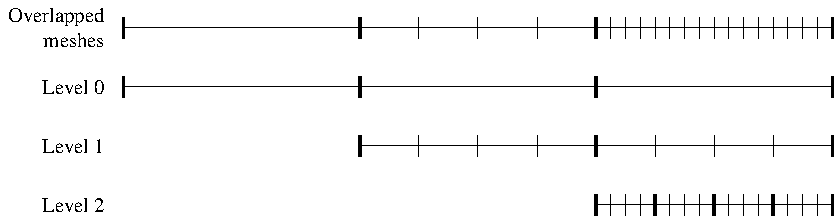
\includegraphics[width=\textwidth]{img/multigrid/multilevel_overlap.pdf}
    \caption{Unfolding of the overlapped hierarchical refinement for a 1D mesh.}
    \label{multilevel_overlap}
\end{figure}

Once defined the spatial refinement, the hanging nodes are included in the algebraic system using \emph{Multi-Point Constraints} (MPC). The values of a hanging node are computed by an average from the father nodes. This operation is performed recursively at all the divisions within the same hierarchic level.

Finally, after the prediction step of a coarse level, its sub-level is advanced with a smaller sub-step. Then, the interface is updated with the values from the prediction and is proceed to compute the solution of the sub-level. This procedure can be executed recursively. Once all the sub-steps have reached the end of the main step, the coarse prediction is updated with the values from the fine level. These steps are resumed in Figure \ref{multilevel_steps}.

\begin{figure} [htpb]
    \centering
    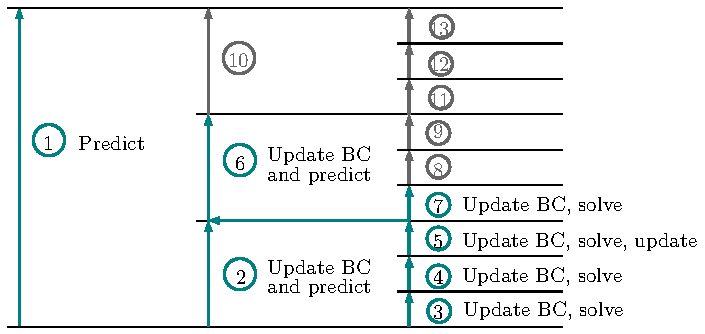
\includegraphics[width=.8\textwidth]{img/multigrid/multilevel_steps.pdf}
    \caption{Steps for solving a coarse time step with hierarchical refinement.}
    \label{multilevel_steps}
\end{figure}

It is important to remark that this procedure does not impose any restriction on having a discontinuity of refinement level higher than one. Regardless of the jump of refinement level, the presented procedure is applied as well.



\section{Data structure}

The hierarchical refinement has been designed in order to be compatible with structured and unstructured meshes. Hence, the data structure is based on a finite element mesh, where nodes are defined by its coordinates and elements are defined by its connectivities.

The refinement begins when some elements are selected to refine according to a criterion which is to be defined. Then, those elements are copied to another mesh container, identified by the consecutive refinement level. The nodes are also copied. It is important to remark that the copied elements are only an auxiliary tool to define the connectivities. The mesh container identified with the refined level might contain elements already refined (Figure \ref{multilevel_meshing_steps}{\color{wrmBlue}a}). During the copying process, the destination nodes save a pointer to the origin node and vice-versa.

Once the coarse connectivities are transferred to the refined mesh, an iterative process begins to refine the elements and conditions until the desired refinement is achieved (Figure \ref{multilevel_meshing_steps}{\color{wrmBlue}b}). Every entity is split by dividing the edges into two. In the case of quadrilaterals, a node is added in the middle of the face, in the case of hexahedra, an extra node is added in the center of the volume. This operation requires some especial attention, because the edges and faces are shared by two elements. For this purpose, an auxiliary variable is defined in order to register the created entities. This variable is a map where the keys are the connectivities of the main edge and the mapped value is the middle node. The iterative process is controlled by the number of divisions executed at every element, each element has a variable storing the number of divisions performed. After executing a division, this value is incremented by one. This process is repeated until the specified number of divisions are reached.

\begin{figure}
    \centering
    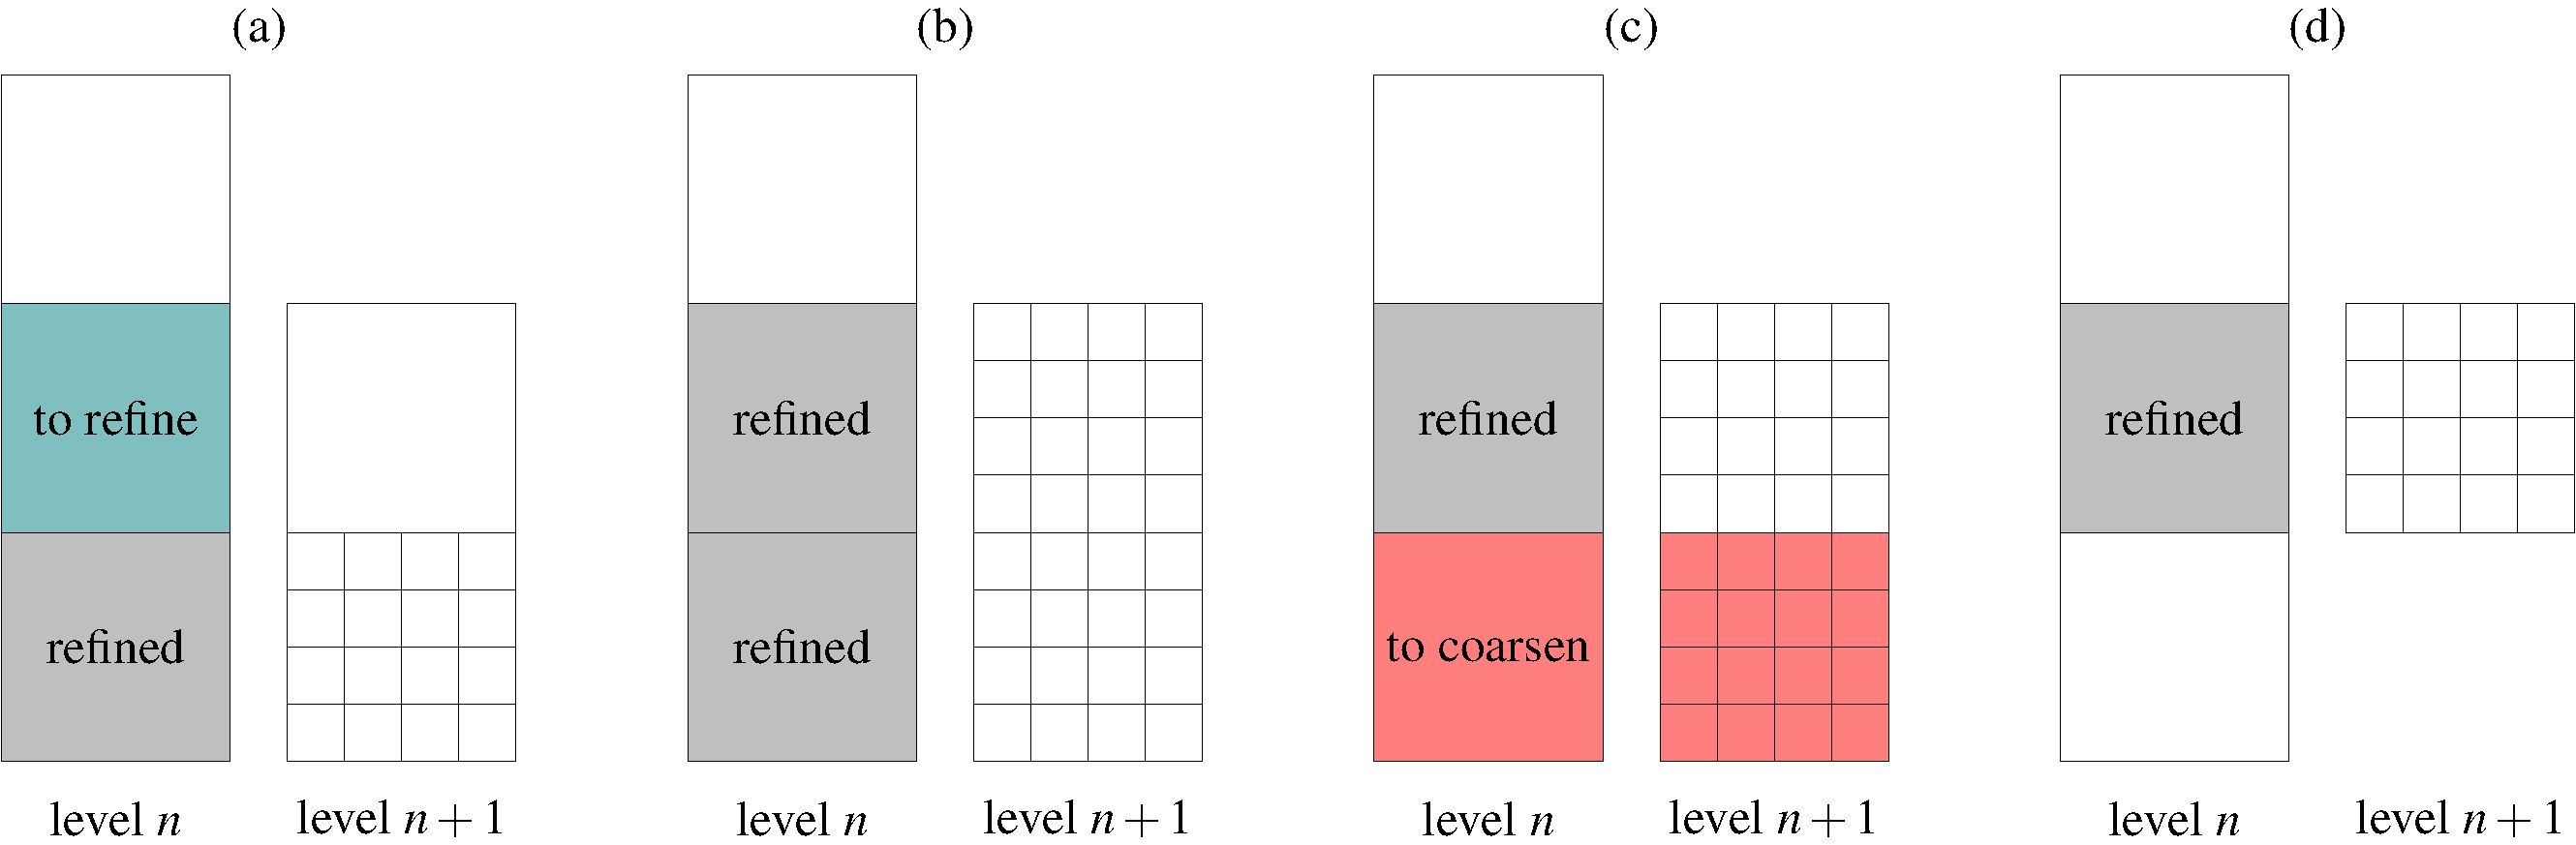
\includegraphics[width=\textwidth]{img/multigrid/multilevel_meshing_steps.pdf}
    \caption{Main steps for the refinement and coarsening process.}
    \label{multilevel_meshing_steps}
\end{figure}

The coarsening process is straightforward. It begins when the refinement criterion marks some elements at the coarse level to coarsen. This information is transferred to the refined elements using an auxiliary variable that allows to map from a refined element to its parent element. Hence, each refined element asks to the parent element if it is to be coarsened (Figure \ref{multilevel_meshing_steps}{\color{wrmBlue}c}).

The coarsening process is done by erasing all the elements to be coarsened from the refined level (Figure \ref{multilevel_meshing_steps}{\color{wrmBlue}d}). The process is finished by cleaning the hanging nodes and the auxiliary variables.
To sum up, the following variables are used by the refinement procedure:
\begin{description}
    \item[LEVEL] Scope: Mesh. The current refinement level.
    \item[REFINED] Scope: Elements, conditions. Flag indicating if the current entity has a nested refinement.
    \item[TO\_REFINE] Scope: Elements, conditions. Flag indicating if it must be refined.
    \item[TO\_COARSEN] Scope: Elements, conditions. Flag indicating if it must be coarsened.
    \item[FATHER\_NODES] Scope: Nodes. If the node is overlapped with a coarse node, there is only one father node and it points to the coarse node. If the current node is refined, it points to the nodes in the refined mesh.
    \item[FATHER\_NODES\_WEIGHTS] Scope: Nodes. The averaging of the nodal values. Has the same size than FATHER\_NODES and the sum of the wights is 1.
    \item[SLAVE\_NODE] Scope: Nodes. It points to a cloned node in the refined mesh.
    \item[FATHER\_ELEMENT] Scope: Elements, conditions. It points to the father entity at he coarse mesh.
    \item[NUMBER\_OF\_DIVISIONS] Scope: Elements, conditions. It counts how many times the entity has been divided.
    \item[NUMBER\_OF\_DIVISIONS] Scope: Mesh. It signifies how many times the entities had to be divided.
    \item[NODES\_MAP] Scope: Mesh. A map pointing to a refined node from the fathers nodes.
\end{description}


This can be easily implemented in parallel with the standard reduction techniques, except the NODES\_MAP. Adding new items to a map in parallel requires some extra architecture to ensure the thread safety. An alternative would be to split this map and reduce its scope to the nodes. This definition has some extra operations to write, read and remove values, but is worth for its scalability.



\section{Refinement criterion}

Finally, the refinement criterion has to be defined. There are two main criteria, the dynamic and the static one. The dynamic depends on the solution after the prediction step. In that case, the residual of the equations is evaluated --it is just the local right hand side when a residual-based system is used-- and compared against a fixed value. When the local residual is too high, the element must be refined if there it has not been already refined. Whenever the local residual is sufficiently small, the element must be coarsened when it has a nested refinement.

The static criterion does not depend on the solution and the mesh is not modified during the analysis. This criterion serves to enhance the quality of the solution in a region. It is important to note that, by its hierarchical definition,  this refinement cannot be used to have a better definition of the boundaries. This algorithm is specially suited for the dynamic criterion.


\section{Examples}


This section includes two basic examples. In the first example is shown how the mesh refinement can help to obtain better solutions. The second example is devoted to test its capabilities in a more complex test with a dynamic meshing.


\subsection{Static refinement}


In this example the propagation os a pulse is analyzed. Let $\Omega=[0,10]\times[0,1]m^2$ be the spatial domain. The initial water depth is $1m$ over all the domain, except near the right boundary, where there is an increment of $1m$.
The initial velocity is null and for $t>0s$ a wave is generated and propagated. Reflective conditions are considered over all the boundary, $\mathbf{u} \cdot \mathbf{n} = 0\ \text{on}\ \Gamma$.

The domain is meshed with a structured triangular mesh of size $0.1m$. In this test a one-level refinement with two division is considered for $y>0.5$. This criterion is static and kept constant during all the simulation. An overview of the mesh and a detail of the refinement is shown in Figure \ref{multilevel_static_mesh}.

\begin{figure} [htb]
    \centering
    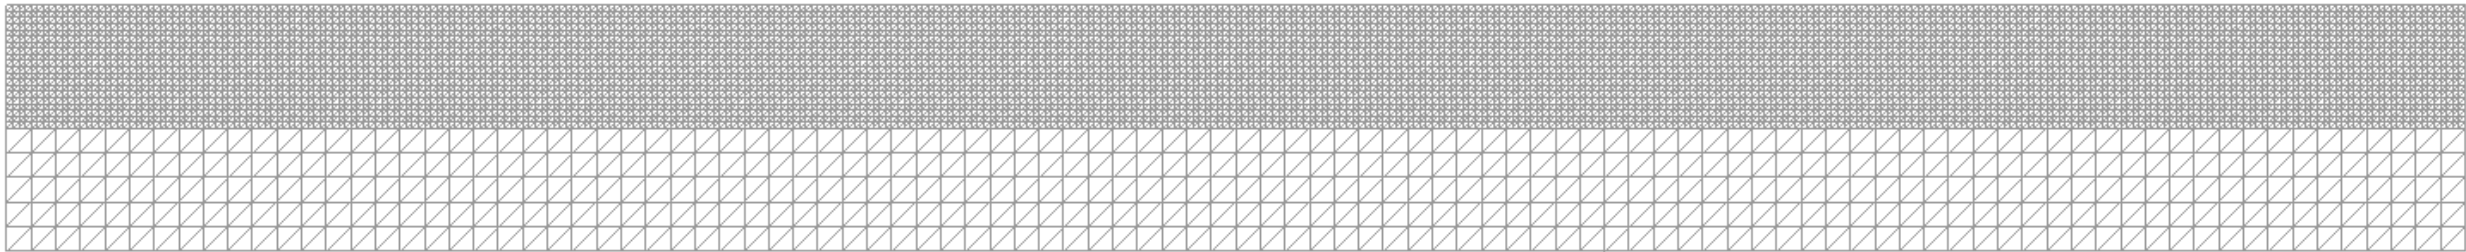
\includegraphics[width=.92\textwidth]{img/multigrid/static/mesh}
    \hfill
    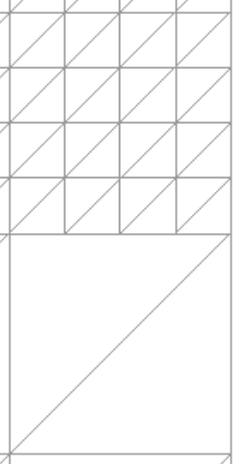
\includegraphics[width=.05\textwidth]{img/multigrid/static/mesh_detail_2}
    \caption{Mesh used for the static refinement test and closeup of the refinement interface.}
    \label{multilevel_static_mesh}
\end{figure}


In Figure \ref{multilevel_static_decoupled} can be appreciated how the solutions obtained at the different regions are very different. In order to magnify this difference, the coarse and the fine domains are decoupled. Firstly, the boundary condition is not updated at the interface from the coarse prediction. Secondly, the coarse solution is not updated with the fine results.


\begin{figure} [htb]
    \centering
    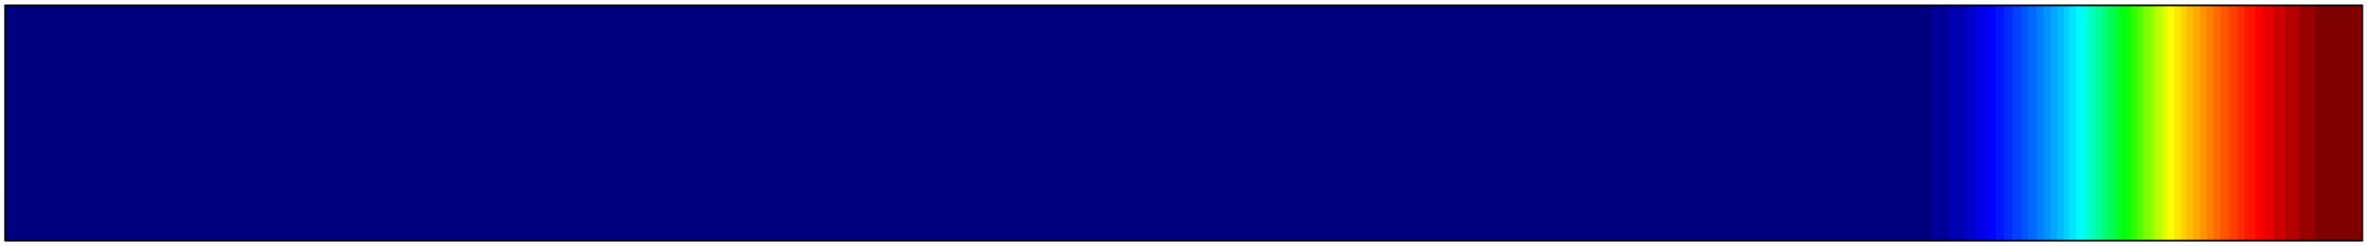
\includegraphics[width=\textwidth]{img/multigrid/static/decoupled-0}\\
    \vspace{5pt}
    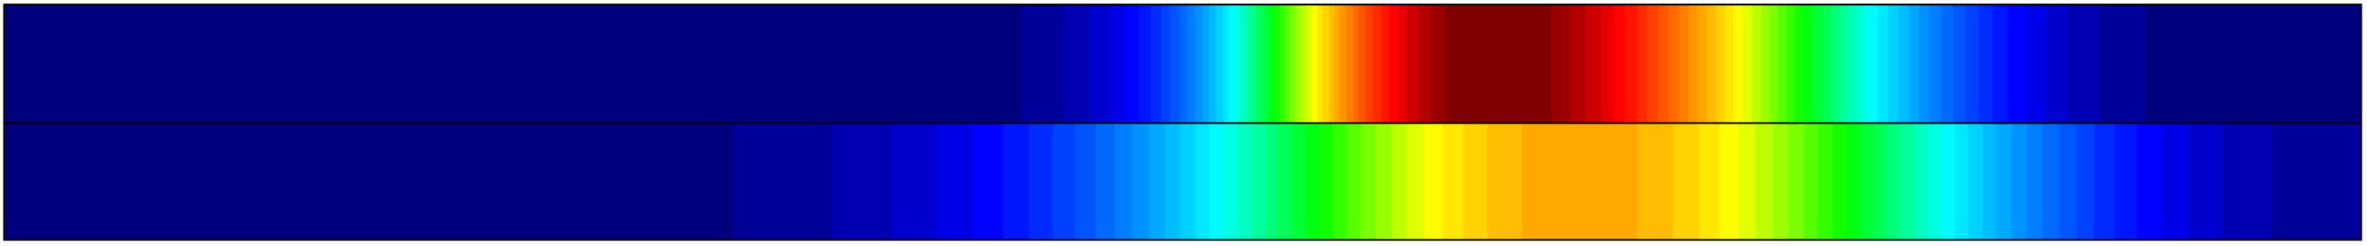
\includegraphics[width=\textwidth]{img/multigrid/static/decoupled-1}\\
    \vspace{5pt}
    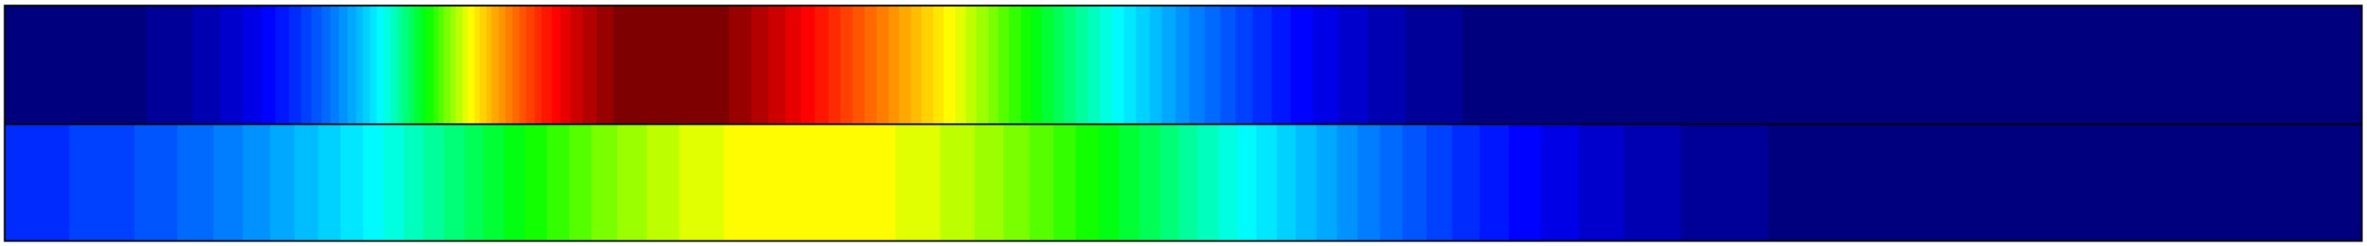
\includegraphics[width=\textwidth]{img/multigrid/static/decoupled-2}
    \caption{Propagation of a pulse with static refinement. Results at time $t=0,1,2s$, The different resolution levels are uncoupled.}
    \label{multilevel_static_decoupled}
\end{figure}


When the two domains are coupled, the information is transferred between the two domains and the solution is modified. In Figure \ref{multilevel_static_coupled} it is possible to appreciate how the wave front is is modified at each sub-domain and how the solution on one sub-domain is modified by the other. For simplicity, the legend is not shown and the contour plot represents only the relative values.

In this test two basic features of the hierarchic refinement are shown. First of all, an accurate discretization is required to obtain an accurate solution without dissipative effects (Figure \ref{multilevel_static_decoupled}). Secondly, the robustness of the data exchange at the interface (Figure \ref{multilevel_static_coupled}).


\begin{figure} [htb]
    \centering
    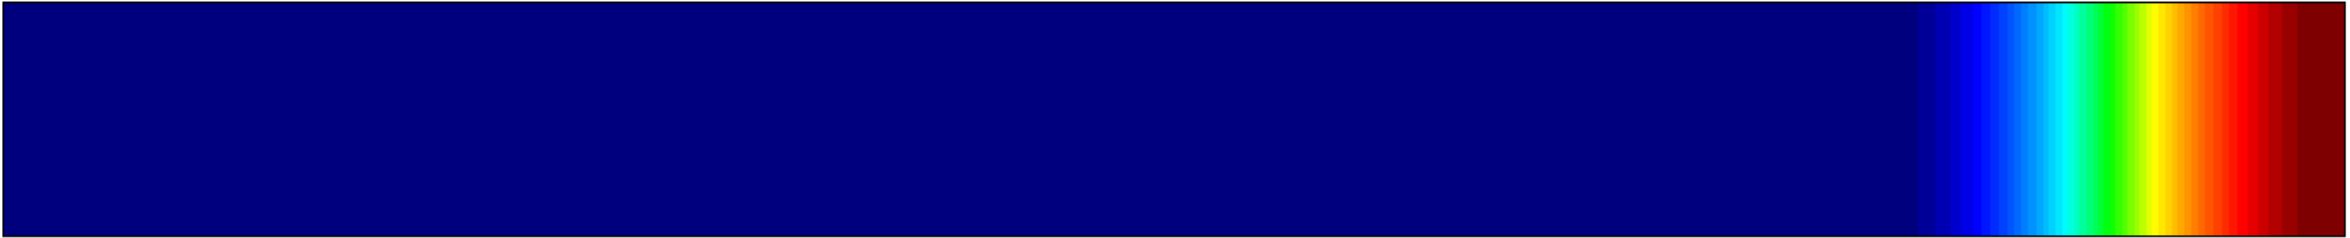
\includegraphics[width=\textwidth]{img/multigrid/static/coupled-0}\\
    \vspace{5pt}
    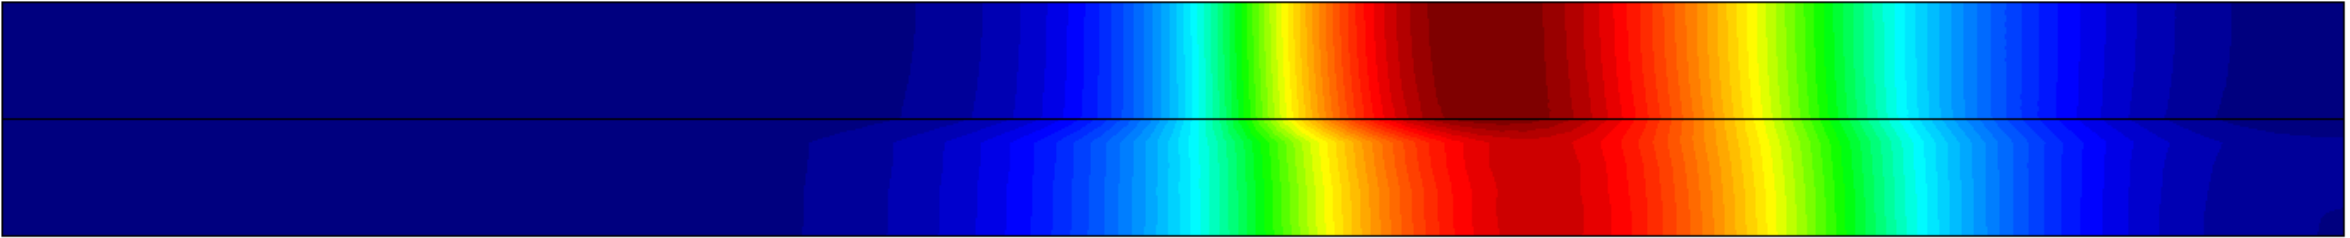
\includegraphics[width=\textwidth]{img/multigrid/static/coupled-1}\\
    \vspace{5pt}
    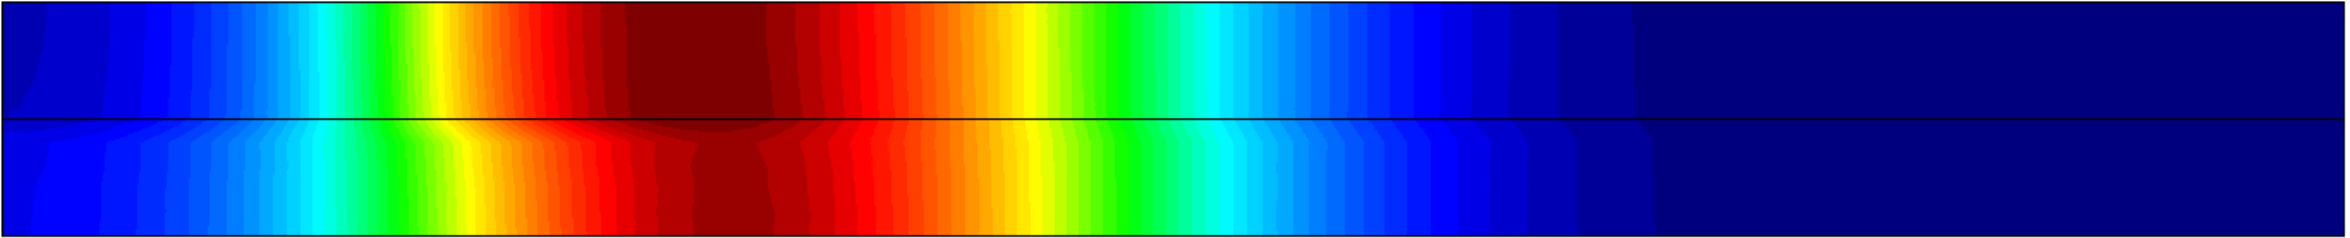
\includegraphics[width=\textwidth]{img/multigrid/static/coupled-2}
    \caption{Propagation of a pulse with static refinement. Results at time $t=0,1,2s$. The different resolution levels are coupled.}
    \label{multilevel_static_coupled}
\end{figure}


\subsection{Dynamic refinement}


The second examples combines the hierarchical refinement with a residual-based criterion. Hence, the resolution level depends on the solution, this fact allows to test the refinement and coarsening processes.

A rectangular domain $\Omega=[0,20]\times[0,10]m^2$ is considered. The mean water depth is $0.1m$ and the solution is initialized with an increment of $0.1m$ at the coordinate $\mathbf{x}_0=(4,3)m$. Reflective conditions are considered over all the boundary, $\mathbf{u} \cdot \mathbf{n} = 0\ \text{on}\ \Gamma$.
After $t=0$ a circular wave is generated, generating reflections at the boundaries which interact with each other.

The domain is initially discretized with an unstructured mesh of triangles of size $0.05m$. A refinement level is added when the local residual is greater than a threshold. When the wave front arrives to a material point, the refinement level is increased and after the wave front has passed, the refinement level is decreased.
Two snapshots of the solution at time $t=10$ and $20s$ are shown in Figure \ref{multilevel_dynamic}.


\begin{figure} [htb]
    \centering
    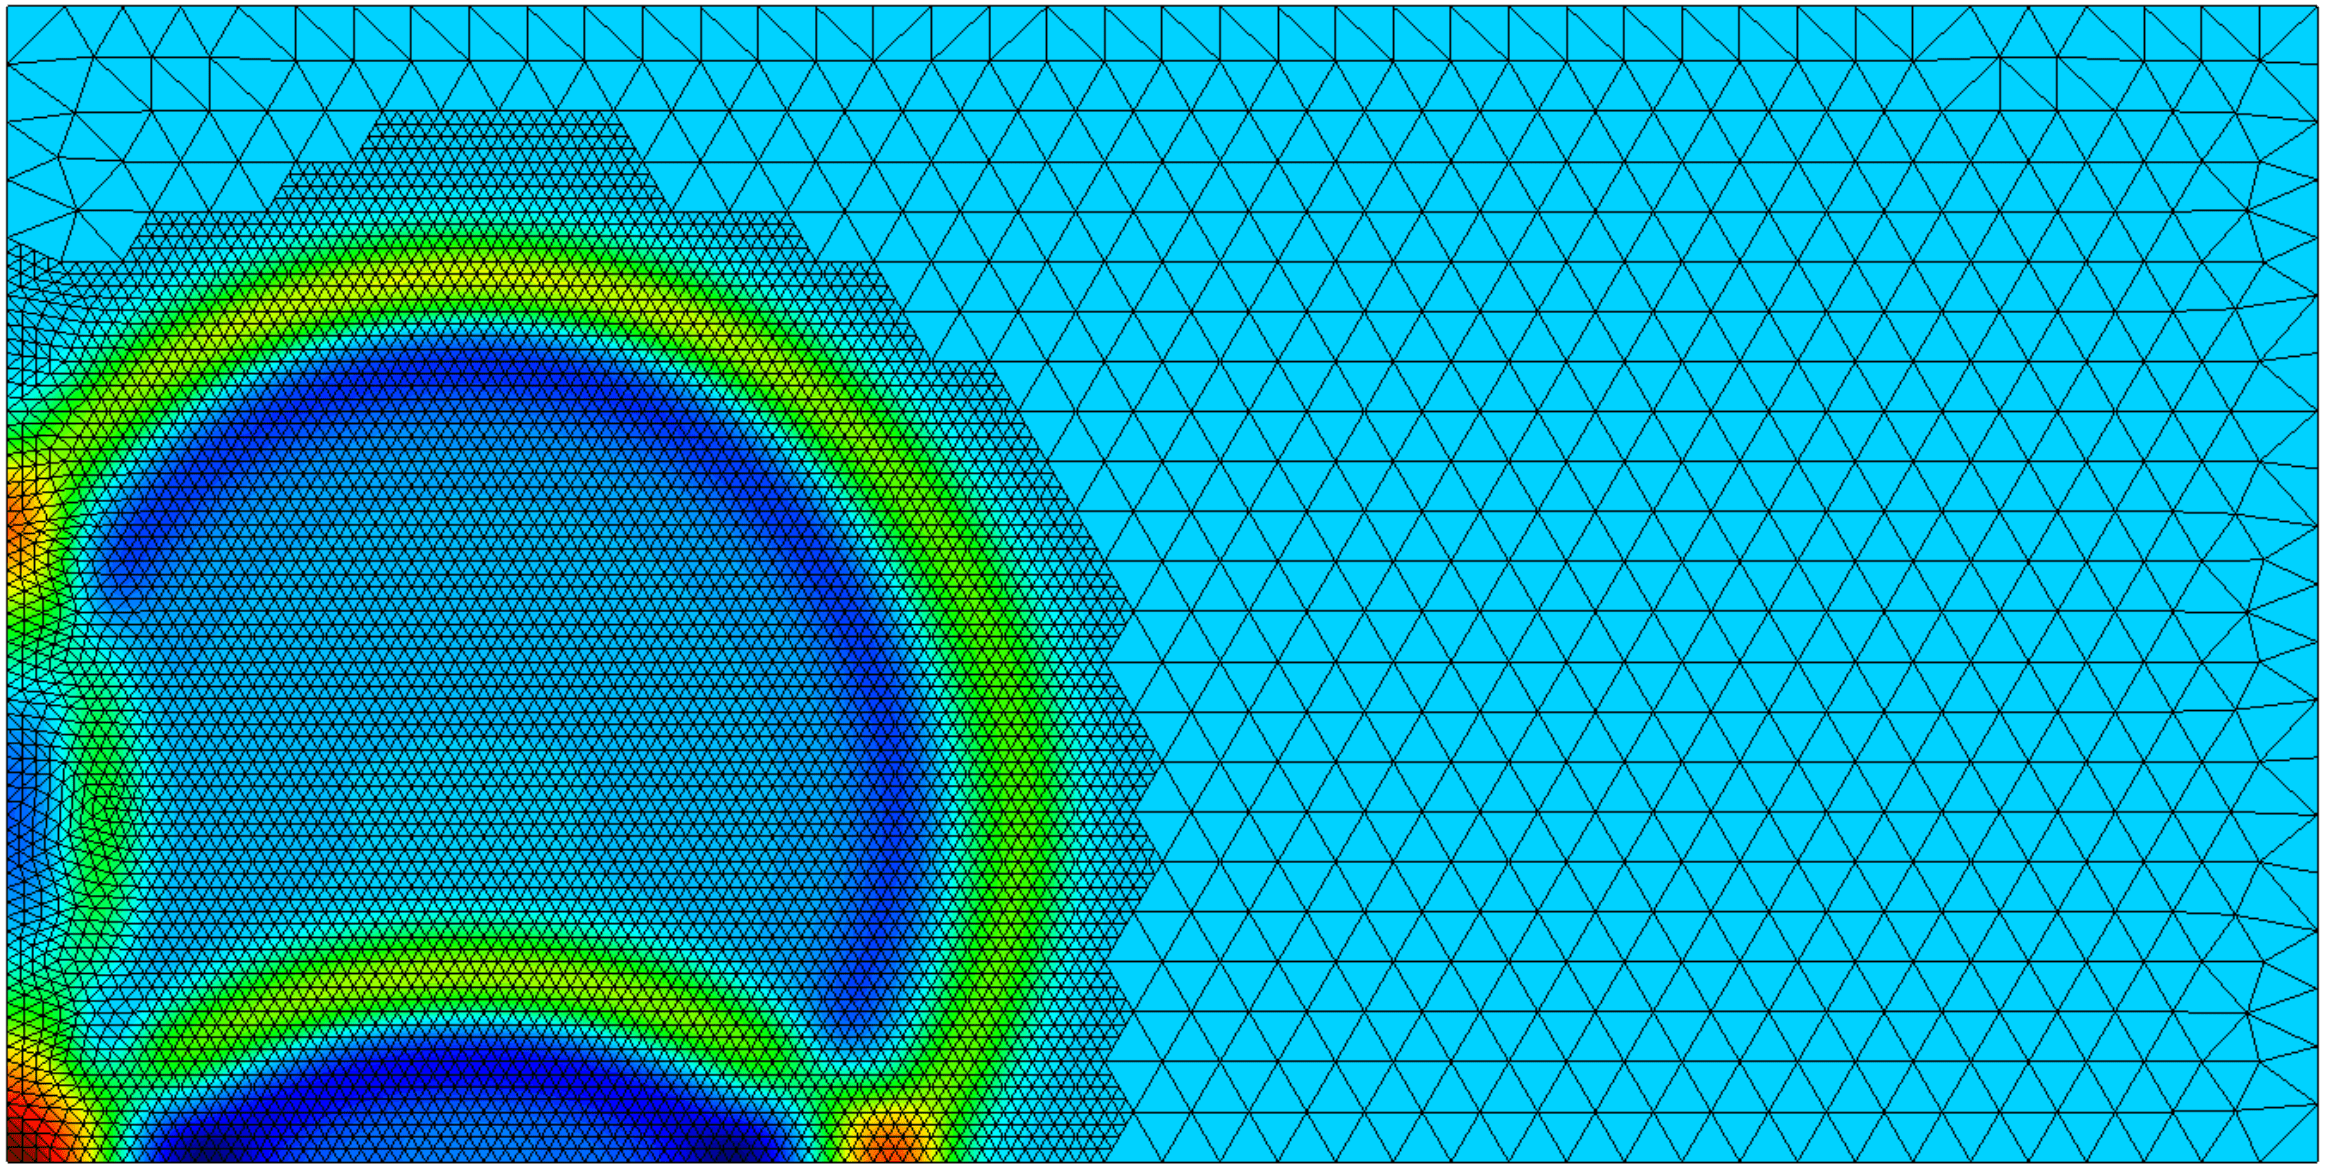
\includegraphics[width=\textwidth]{img/multigrid/dynamic/dynamic-10-min}\\
    \vspace{5pt}
    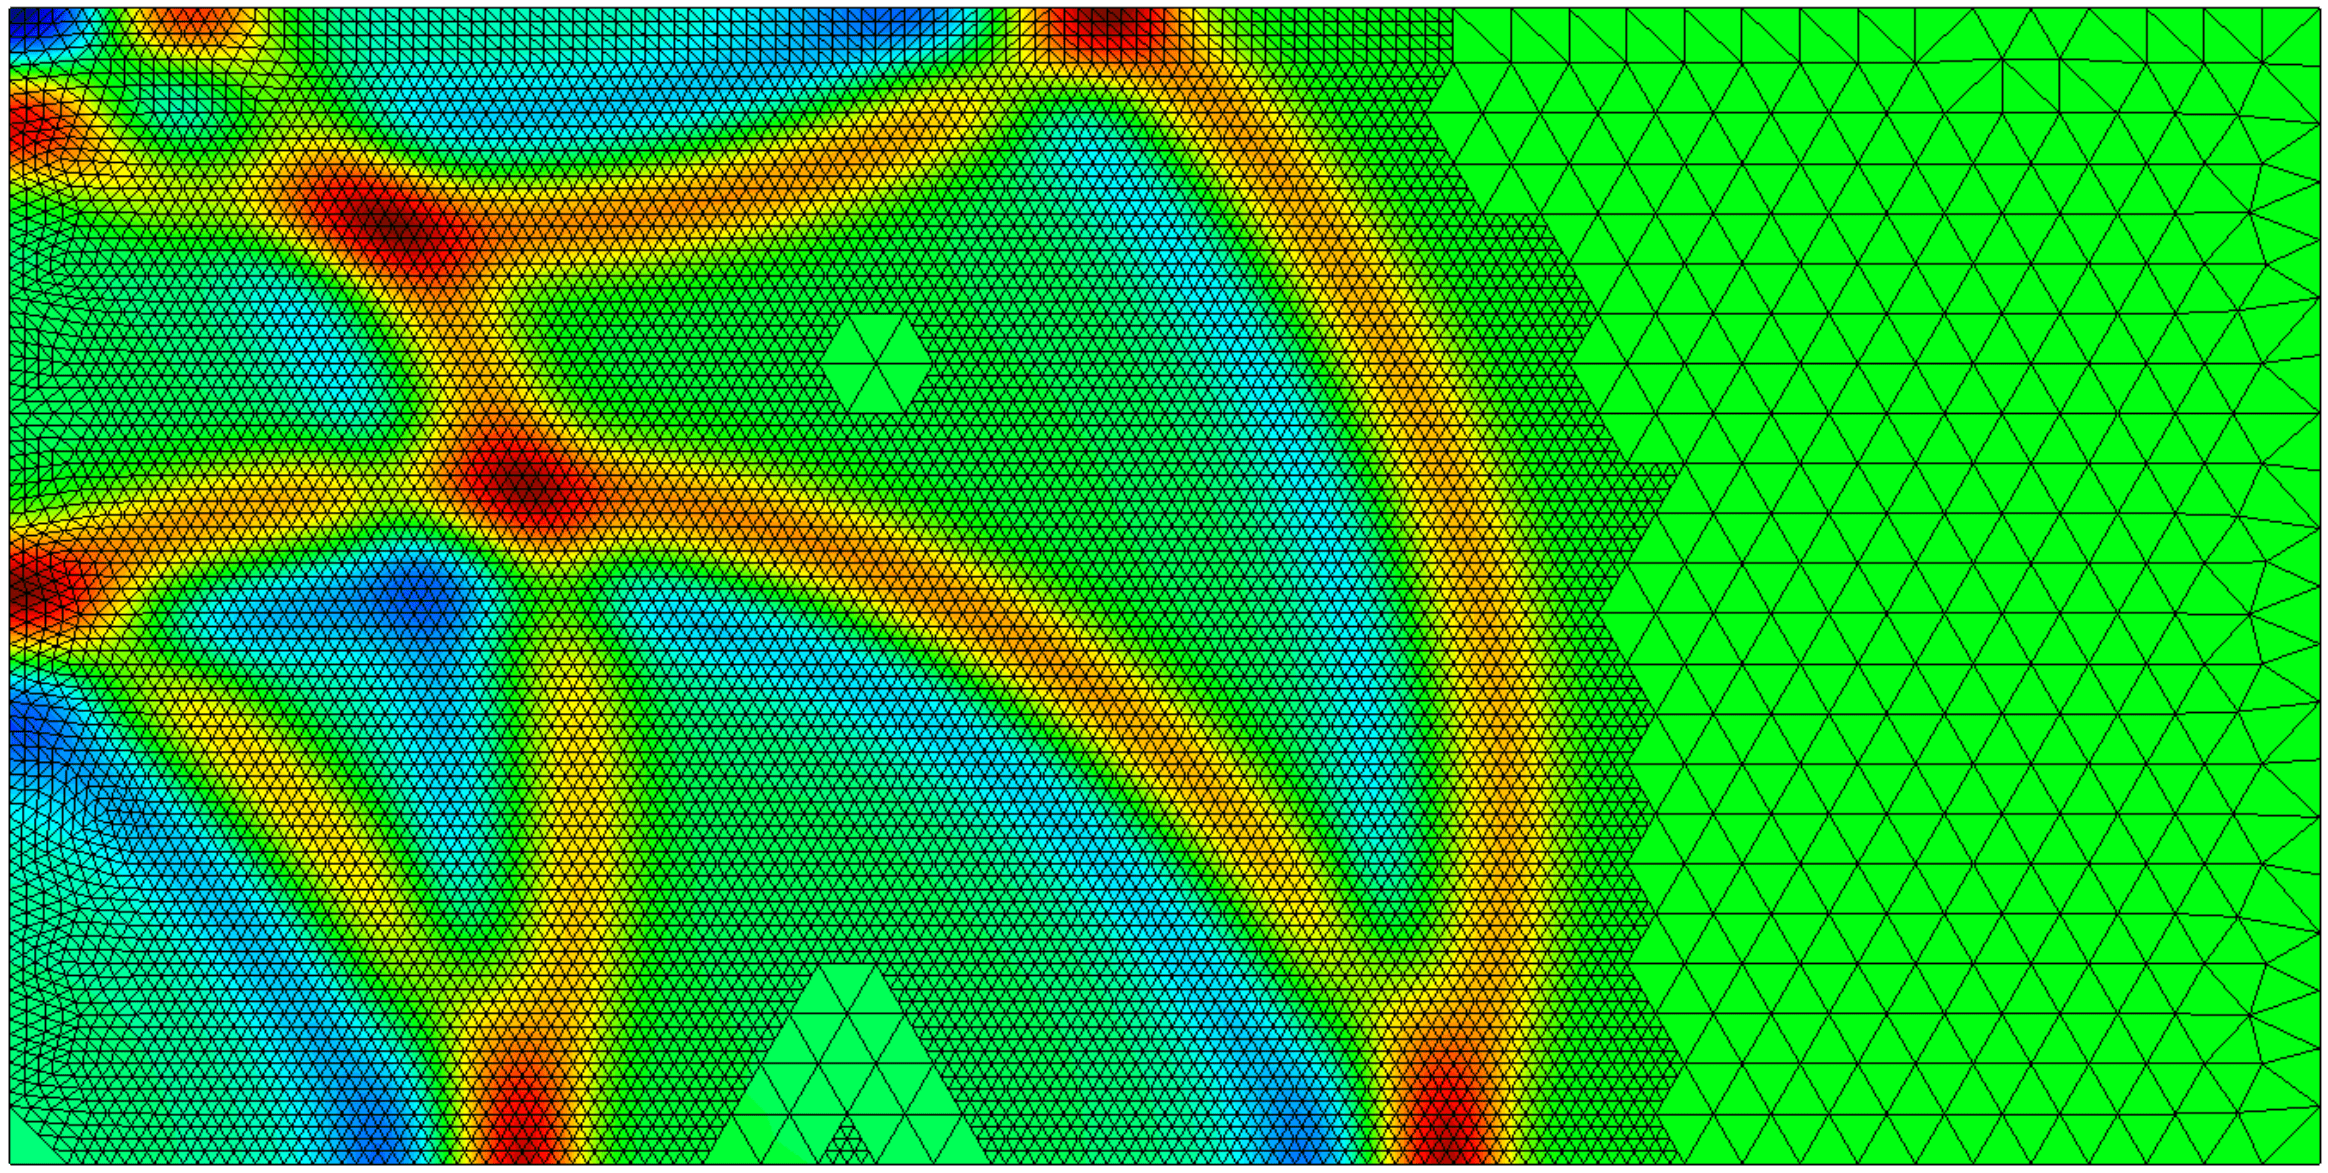
\includegraphics[width=\textwidth]{img/multigrid/dynamic/dynamic-20-min}
    \caption{Propagation of a wave with a dynamic refinement. Results at time $t=10$ and $20s$. The different resolution levels are coupled.}
    \label{multilevel_dynamic}
\end{figure}


\section{Conclusions}


The basic structure of a hierarchical refinement with LTS has been presented in this appendix. The design of the local refinement with LTS is decoupled from the time integration scheme, this is achieved with an overlap of the fine domain with the coarse one. This fact allows to use arbitrarily an explicit or implicit time step without compromising the stability of the method near the fine interface.

Despite duplicating the coarse degrees of freedom at the refined sub-domain, the computational requirements are not increased. The computation of the duplicated degrees of freedom represents $1/64$ over the cost of the fine solution, when two divisions are made. The duplicated degrees of freedom are part of a prediction step which is used to specify the boundary conditions at the interface during the sub stepping of the lower level. Moreover, this design extremely simplifies the refinement and coarsening procedures.

This type of refinement is specially interesting when obtaining an accurate solution is linked to a fine discretization in a small part of the domain. The hierarchical mesh refinement can be applied recursively in order to obtain several levels of accuracy depending on the quality of the solution.


